\newpage
\section{Implementacja}
Do implementacja naszego algorytmu zdecydowaliśmy się wykorzystać język programowania Python.\\

\subsection{ Wykorzystywane biblioteki }\\

Wykorzystano następujące biblioteki języka Python: \\
\begin{itemize}
    \item termcolor - do pokazywania logów w konsoli w kolorze zielonym - kiedy test przebiegł pomyślnie oraz w kolorze czerwonym - kiedy pojawił się błąd
    \item tqdm - wyświetla progres wykonywania zadania w naszych przypadku, na jakim poziomie jest obecnie wykonywany test
    \item Crypto.Cipher - tej biblioteki użyliśmy do szyfrowania szyfrem AES
\end{itemize}\\


\subsection{ Uruchomienie symulacji  }
Do uruchomienia programu realizującego zadane symulacje wymagany jest \textbf{Python 3} oraz zainstalowanie powyższych zależności. Zostały one zawarte w pliku \textit{requirements.txt.} Należy je zainstalować za pomocą polecenia: \textbf{\textit{pip install -r requirements.txt}} Aby uruchomić symulację należy wewnątrz folderu wywołać w konsoli polecenie \textbf{\textit{python tests.py.}}\\

\subsection{ Implementacja  }
Implementacja naszego algorytmu składa się z 3 plików:\\
\begin{itemize}
    \item SM4.py
    \item tests.py 
    \item bytesHelpers.py
\end{itemize}\\

\newline W pliku bytesHelpers umieszczone zostały funkcje pomocniczne tj. long\_to\_bytes, bytes\_to\_long, xor oraz leftShift. \\

Plik SM4.py opisuję główną klasę algorytmu, składa się z następujących elementów, które realizują schemat algorytmu przedstawiony w punkcie 3:

\begin{itemize}
\setlength\itemsep{1.2em}
    \item \textbf{konstruktora} - tworzy obiekt klasy SM4, składający się z klucza (\textit{key}), oraz zmiennej \textit{roundedKeys}, która przechowuje 32 klucze rund oraz zmiennej \textit{recentOutputs}, która przetrzymuje wartość wyjściową z danej rundy i przekazuje ją na wejście kolejnej rundy
    \item \textbf{stałych}: 
    \begin{itemize}
    \setlength\itemsep{1em}
        \item [$\diamond$] \textit{sboxTable} - skrzynka podstawieniowa
        \item [$\diamond$] \textit{FK} - parametr FK
        \item [$\diamond$] \textit{CK} - parametr CK
    \end{itemize}
    \item \textbf{funkcji}: 
    \begin{itemize}
    \setlength\itemsep{1em}
        \item [$\diamond$] \textit{getRoundKeys} - pobiera wektor kluczy
        \item [$\diamond$] \textit{getRecentOutputs} - pobiera wartość \textit{recentOutputs}
        \item [$\diamond$] \textit{encrypt} - funkcja szyfrująca, wywołuje funkcje \textit{encryptDecrypt} z przekazywanym tekstem do zaszyfrowania
        \item [$\diamond$] \textit{decrypt} - funkcja deszyfrująca, wywołuje funkcje \textit{encryptDecrypt} z przekazywanym tekstem do odszyfrowania oraz drugim parametrem \textit{isDecryption} ustawionym na \textit{true}
        \item [$\diamond$] \textit{encryptDecrypt} - w zależność od typu operacji: szyfrowanie lub deszyfrowanie ustawia odpowiednią kolejność kluczy, dzieli tekst na 4 słowa i wywołuje 32 razy funkcję rundy\textit{roundFunction}
        \item [$\diamond$] \textit{roundFunction} - wykonuje operacje XOR z wyjściem funkcji \textit{mixerSubstitution}
        \item [$\diamond$] \textit{mixerSubstitution} - wywołuje liniowanie przekształcenie (\textit{linearSubstitution}) podając jako parametr wyjście funkcji nieliniowego przekształcenia (\textit{nonlinearSubstitution})
        \item [$\diamond$] \textit{nonlinearSubstitution} - generuj wektor z 4 słów, które zostały stworzone przy pomocy skrzynki podstawieniowej
        \item [$\diamond$] \textit{linearSubstitution} - wykonuje serie operacji XOR z wektorami po rotacji w lewo, odpowiednio o 2, 10, 18 i 24 bity.
        \item [$\diamond$] \textit{keyExpansion} - generuje 32 klucze dla każdej rundy poprzez XORowanie poszczególnych słów klucza z odpowiednimi elementami \textit{parametru FK}, następnie w pętli dodaje je do listy jednocześnie XORując wcześniejszy klucz z wyjściem funkcji \textit{mixerSubstitution2}
        \item [$\diamond$] \textit{mixerSubstitution2} - wywołuje liniowanie przekształcenie (\textit{linearSubstitution2}) podając jako parametr wyjście funkcji nieliniowego przekształcenia (\textit{nonlinearSubstitution})
        \item [$\diamond$] \textit{linearSubstitution2} - XORuje wektor z wektorami po rotacji w lewo, odpowiednio o 13 i 23 bity.
        \item [$\diamond$] \textit{sbox} - zwraca podstawiony wektory przy pomocy skrzynki podstawieniowej - \textit{sboxTable}
    \end{itemize}
\end{itemize}\\

Wszelkie powyższe operacje są dokładną implementacją operacji występujących w algorytmie SM4.


\subsection{ Testy  }

Testy zrealizowany zostały przy pomocy pliku \textit{tests.py}. Przykłady scenariuszy testowy:\\
\begin{enumerate}
    \item Sprawdzenie, czy klucze wygenerowały się poprawnie i są takie jak oczekiwaliśmy. \\
    \item Zaszyfrowanie jednego słowa i porównanie, czy wyniki jest zgodny z oczekiwanym.\\
    \item Odszyfrowanie jednego słowa i porównanie, czy wyniki jest zgodny z oczekiwanym.\\
    \item Testy wykonane w pętli dla 1000000 iteracji. Po każdej iteracji sprawdzenie, czy tekst został zaszyfrowany poprawnie.
    \item Testy wykonane w pętli dla 1000000 iteracji. Po każdej iteracji sprawdzenie, czy tekst został zdeszyfrowany poprawnie.\\
\end{enumerate}


Dodatkowo, aby przeprowadzić porównanie wydajnościowe z algorytmem AES, przeprowadziliśmy dodatkowe testy.\\
\begin{enumerate}
    \item Zaszyfrowanie jednego słowa i porównanie, czy wyniki jest zgodny z oczekiwanym dla algorytmu AES.\\
    \item Odszyfrowanie jednego słowa i porównanie, czy wyniki jest zgodny z oczekiwanym dla algorytmu AES.\\
    \item Testy wykonane w pętli dla 1000000 iteracji. Po każdej iteracji sprawdzenie, czy tekst został zaszyfrowany poprawnie dla algorytmu AES.\\
    \item Testy wykonane w pętli dla 1000000 iteracji. Po każdej iteracji sprawdzenie, czy tekst został zdeszyfrowany poprawnie dla algorytmu AES.\\
\end{enumerate}



Wszystkie testy przebiegły pomyślnie, co potwierdza poniższy zrzut ekranu.

\begin{figure}[H]
  \centering
  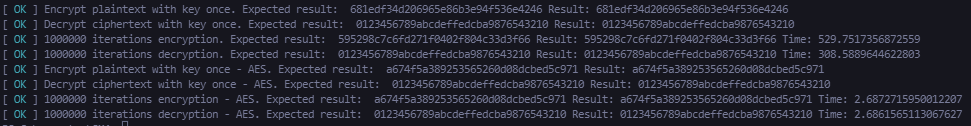
\includegraphics[scale=0.7]{diagramy/testy.PNG}
  \caption{Testy algorytmu szyfrowania SM4}
  \label{fig:SM4}
\end{figure}

\subsection{ Porównanie wydajności }

Planem analizy wydajności, było przeprowadzanie takie samej liczby testów, z tym samym słowem i kluczem, dla algorytmu SM4 oraz AES, ponieważ oba te algorytmy to szyfry blokowe. Aby to zrobić zmierzyliśmy czas wykonywania wszystkich iteracji dla każdego algorytmu i wyliczyliśmy średnia przepływność tych algorytmów. Otrzymane wyniki zaprezentowaliśmy w tabeli  \ref{table:AES_to_SM4}.

\begin{table}[h!]
\centering
\caption{Porównanie przepływności}
\label{table:AES_to_SM4}
\begin{tabular}{ | c | c | c | } 
\hline
 Metoda & Algorytm SM4 [MB/s]& Algorytm AES [MB/s] \\
\hline
$Szyfrowanie$ & 0,03 & 5,68 \\
$Deszyfrowanie$ & 0,05 & 5,68\\
\hline
\end{tabular}
\end{table}

Algorytm AES jest zdecydowanie szybszym algorytmem niż algorytm SM4, ponad 100-krotnie. Fakt, że algorytm SM4 nie został jeszcze złamany, świadczy o jego atrakcyjności ze względu na poziom bezpieczeństwa, jednak pod względem wydajności, w przypadku naszej implementacji, zdecydowanie lepiej prezentuje się algorytm AES. Tak duża różnica w wydajności może być spowodowana implementacją SM4 w języku Python, który jest językiem interpretowanym. Z dużym prawdopodobieństwem lepsze rezultaty uzyskałaby implementacja w języku kompilowanym takim jak np. C.